\section{Method}
\label{sec:method}

\begin{figure*}[t]
 \centering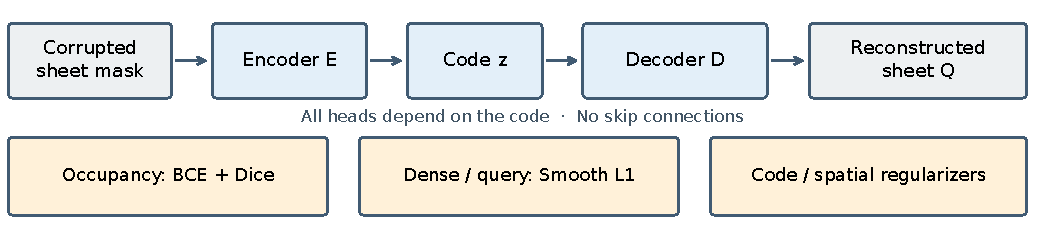
\includegraphics[width=\textwidth]{figures/ae.pdf}
 \caption{\textbf{Learn the sheet space.} Reconstruct a clean sheet from a
 corrupted mask through a latent bottleneck. Auxiliary distance heads and
 regularizers shape the representation. After training, freeze the AE.}
 \label{fig:ae}
\end{figure*}

\begin{figure*}[t]
 \centering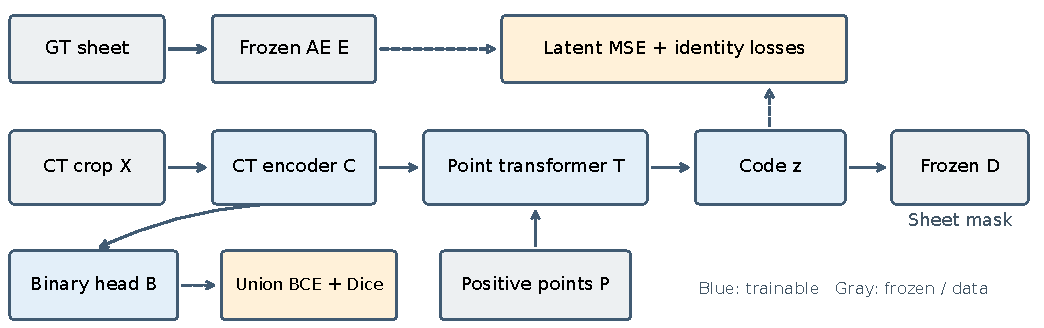
\includegraphics[width=\textwidth]{figures/training.pdf}
 \caption{\textbf{Learn point-to-sheet prediction.} CT and positive points
 predict the frozen AE's sheet code. The binary branch jointly supervises
 CT features; the new automatic recipe also uses it for seed proposal.
 Blue modules are trained; gray modules are frozen or inputs.
 The frozen sheet decoder produces the final mask at inference.}
 \label{fig:training}
\end{figure*}

PLatS first learns a single-sheet code, then predicts it from CT and points.
At inference, the same code space supports prompted reconstruction and
automatic instance discovery. Detailed modules and losses are in Supplementary.

\subsection{Learn a sheet representation}
An autoencoder learns to reconstruct a clean sheet mask $S$ from its corrupted
version $\widetilde S$:
\begin{equation}
 z=E(\widetilde S),\qquad Q=\sigmoid(D(z)).
 \label{eq:aesimple}
\end{equation}
$E$ is the sheet encoder, $z$ its latent code, $D$ the occupancy decoder,
and $Q$ the reconstructed probability map; $\sigmoid$ is the sigmoid function.
There are no encoder--decoder skip connections: the shape must pass through
$z$ (Fig.~\ref{fig:ae}). Occupancy heads use BCE and Dice losses;
dense and point-query distance heads use Smooth L1 supervision.
Different-sheet code repulsion and outside-sheet/border penalties regularize
training. Exact heads, noise and loss weights are in Supplementary.
No explicit topology loss is used.

\subsection{Predict the code from CT and points}
CT encoding and image-context blocks $C$ extract a shared feature grid. A transformer $T$ combines
these features with a set of positive points $P$ to predict a sheet code:
\begin{equation}
 \widehat z=T(C(X),P),\qquad
 \widehat S=\mathbf1[\sigmoid(D(\widehat z))\ge 0.5].
 \label{eq:predictsimple}
\end{equation}
$X$ is the CT crop, $\widehat z$ the predicted code, $\widehat S$ the binary
sheet prediction, and $\mathbf1$ the indicator function.
We train code prediction with MSE against the frozen AE's clean-sheet code;
normalization is omitted here for clarity and defined in Supplementary.
Same-sheet and different-sheet losses encourage consistent instance identity.
A co-trained binary decoder $B$ shares the CT encoder and image context,
then predicts the sheet union with BCE and Dice supervision
(Fig.~\ref{fig:training}). The new training recipe crops only before the final
upsampling stage, retaining earlier full-volume decoder context.
The AE remains frozen, and the main point-to-sheet model needs no decoded
occupancy loss during training.
Prompt conditioning and latent prediction operate on a $10^3$ grid for a
$320^3$ crop; full sheet decoding is deferred until a mask is needed.
Supplementary details the modules, supervision and computational scope.

\subsection{Discover instances automatically}
Encode CT once and use the co-trained binary decoder to propose foreground
seeds. Reuse the cached CT context to predict one code per seed, then cluster
nearby codes using full-code MSE. For each retained
cluster, combine consistent multi-point predictions and decode a sheet.
Remove small components and duplicates, then assign overlapping voxels by
predicted probability. Figure~\ref{fig:inference} shows an actual example.
The reported automatic benchmark fixes a separate foreground proposer and
512 seeds per crop to control inputs across checkpoints; its measured outputs
are retained in Fig.~\ref{fig:inference}. The co-trained proposal path is the
new recipe and has not been benchmarked here. Thresholds and exclusions are
in Supplementary. Raw prompted topology is measured before cleanup.

\begin{figure*}[t]
 \centering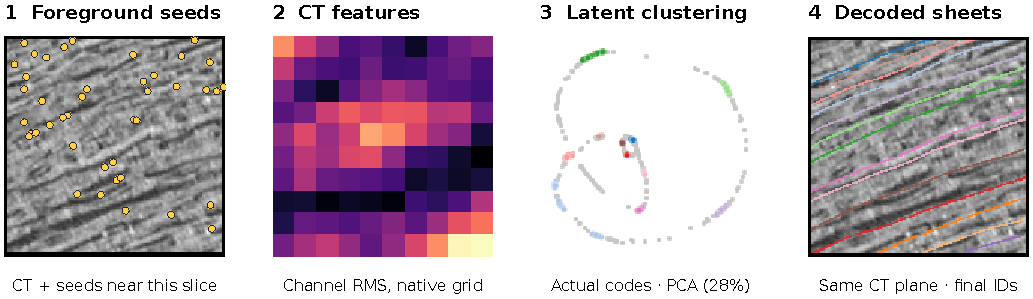
\includegraphics[width=\textwidth]{figures/inference.pdf}
 \caption{\textbf{Automatic inference on a real CT crop.}
 Left to right: foreground seeds, cached CT features, predicted codes grouped
 by identity, and decoded instances. The CT and output use the same native
 $z$ slice of case 00860. The code plot is a 2D PCA display of all 512 measured
 codes; clustering uses their full dimension. Gray points are discarded.
 Colors link retained codes to final sheet IDs. See Supplementary for display details.}
 \label{fig:inference}
\end{figure*}
